% Drawing 154/03-1 -- folder 154, batch 03, archive page 43 (PDF page 44).
% Transcription: figure dans le texte de e) : un segment vert foncé sur $K$, ses deux extrémités relevées en vert clair, l'une marquée d'un point noir et d'une étoile de traits orange ; trois traits orange en pointillé traversent le segment
% Kind: segment of K with raised ends. Method 2 (schematic redraw from the facsimile). Status: ok.
% Notes: In the text of e): a dark green segment on K, its two ends raised in light green; the black point is at the right end of the segment (where it turns up), and the star of orange strokes sits on the top of the raised right end; three dotted orange strokes cross the segment.
% Coordinates: 1 unit = 1 mm = 1/100 of the crop width (bbox in page fractions: [0.479, 0.425, 0.565, 0.467]).
% Redrawn by Claude (claude-opus-5-5), issue #73, 2026-11-07; not checked by a human; not compiled (no TeX in the session).
% Rights: reproduces part of the work -- behind RENDER_TRANSCRIPTS, never published by itself.
\documentclass[tikz,border=3pt]{standalone}
\usepackage{amsmath,amssymb}
\usetikzlibrary{patterns,arrows.meta}
\tikzset{Or/.style={orange!90!black}, Ye/.style={yellow!80!orange}, Lg/.style={green!60!black!70}, Dg/.style={green!45!black}, Br/.style={brown!80!black}, Rd/.style={red!85!black}, Bl/.style={blue!70!black}, Gy/.style={black!40}, pencil/.style={black!45}, struck/.style={black!35}, mark/.style={circle,draw,inner sep=1.3pt}, pt/.style={circle,fill,inner sep=0.9pt}, opt/.style={circle,draw,fill=white,inner sep=1.1pt}}
\begin{document}
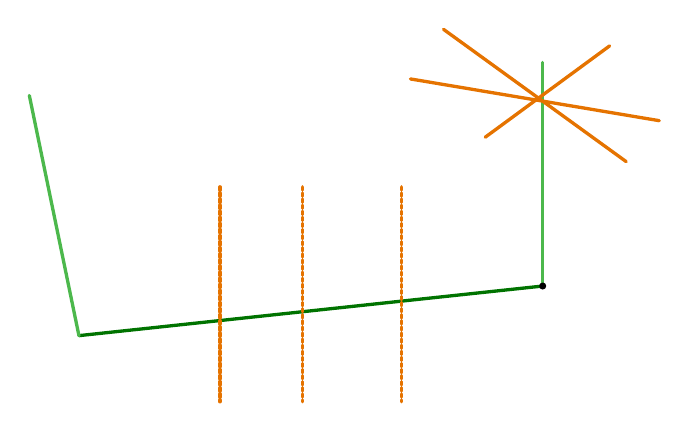
\begin{tikzpicture}[x=1mm,y=1mm,line cap=round,line join=round,font=\scriptsize]
\draw[Dg,very thick] (13.7,-50.5) -- (72.6,-44.2);
\draw[Lg,very thick] (13.7,-50.5) -- (7.4,-20);
\draw[Lg,very thick] (72.6,-44.2) -- (72.6,-15.8);
\node[pt] at (72.6,-44.2) {};
\draw[Or,very thick] (55.8,-17.9) -- (87.4,-23.2);
\draw[Or,very thick] (60,-11.6) -- (83.2,-28.4);
\draw[Or,very thick] (65.3,-25.3) -- (81.1,-13.7);
\draw[Or,densely dotted,very thick] (31.6,-31.6) -- (31.6,-58.9);
\draw[Or,densely dotted,very thick] (42.1,-31.6) -- (42.1,-58.9);
\draw[Or,densely dotted,very thick] (54.7,-31.6) -- (54.7,-58.9);
\end{tikzpicture}
\end{document}
